\documentclass[11pt]{article} 

\usepackage{graphicx}
\usepackage{lineno}
\usepackage{enumitem} 
\usepackage{lscape}
\usepackage{hyperref} 
\usepackage{apacite}
\usepackage{booktabs}
\usepackage{adjustbox}
\usepackage{subcaption}

\begin{document}


\begin{center}

\includegraphics[scale=0.52]{mmulogo.jpeg}\\
\vspace{0.5cm}
\Large{\textbf{TDS 3301 \\DATA MINING}} \\
\vspace{1.5cm}
\Large{\textbf{PROJECT}} \\
\vspace{1cm}
\large{\textbf{QUESTION 3: Intelligent Decision-Making for Loan Application}}
\vspace{1cm}
 


\vspace{5cm}


\normalsize{Prepared by} \\
\vspace{1cm}
\large{\textbf{Ong Shuoh Chwen, 1171102212, 018-2992362}} \\ 
\large{\textbf{Yong Wen Kai, 1171101664, 016-3963254}} \\ 
 

\end{center}

\thispagestyle{empty}
\pagenumbering{gobble} 
\clearpage 
\setcounter{page}{0}
\tableofcontents
% ============================================

\clearpage
\pagenumbering{arabic}
\setcounter{page}{1}
\section{Exploratory Data Analysis (EDA)}
The dataset used in this project is from Question 3: Intelligent Decision-Making for Loan Application, \textit{'Banking\_CS.csv'}. The dataset contained the basic personal data of the person applying for loan, ranging from employment type, loan amount, credit card type and etc.

The EDA process starting off by with filling in the missing values of the data, pre-processing the data, oversampling the data, and performing the EDA tasks to understand the data even more in-depth and better.

\subsection{Missing Values Treatment}
\subsubsection{Checking for missing values}
First and foremost, empty or missing values are required to be either get rid off or replace by assigning new values to it. In this section, we are going to use \textit{isnull()} function to check if there's any missing or null values in the dataset. 

\begin{figure}[h]
\centerline{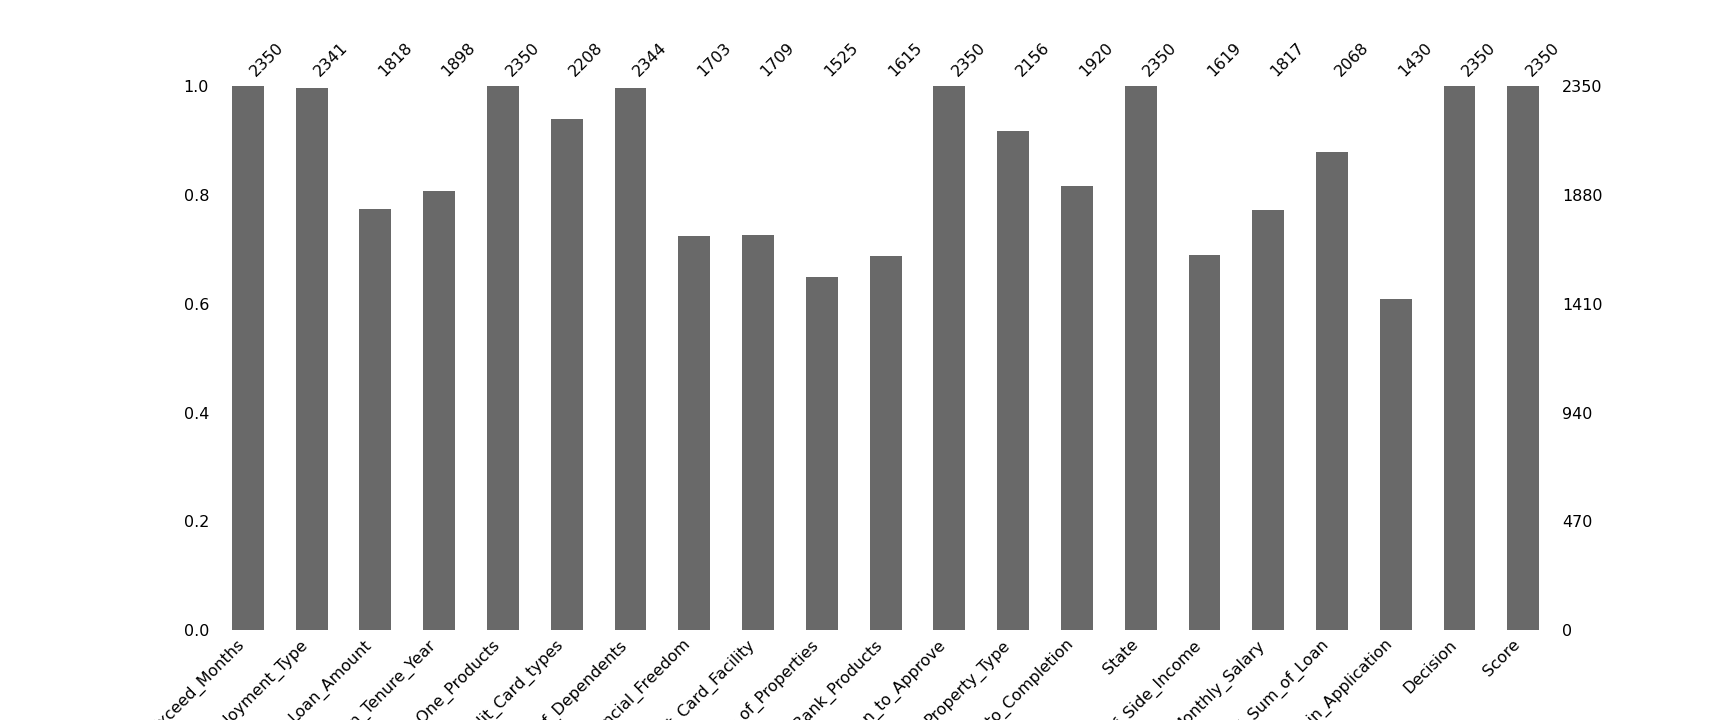
\includegraphics[scale=0.2]{missing_val.png}}
\caption{The results of \textit{isnull()}}
\label{fig:isNull}
\end{figure}

Based on Figure ~\ref{fig:isNull}, we found out that the dataset contained a lot of missing values, such as Loan\_Amount, Loan\_Tenure\_Year, Credit\_Card\_types, Years\_to\_Financial\_Freedom, Card\_Facility, Number\_of\_Properties, Property\_Type, Years\_for\_Property\_to\_Completion, Number\_of\_Side\_Income, Monthly\_Salary, Total\_Sum\_of\_Loan and Total\_Income\_for\_Join\_Application.

\clearpage
\subsubsection{Dealing with missing values}
From the missing values we found in the previous subsection, we are going to fill those missing values with mode values from each corresponding column. We felt that removing those missing values are going to impact hard on the upcoming data preprocessing, as some of the data are very limited. For instance, data from Kedah state are 1 out of 10 compared to Johor state which are almost 8 out of 10. 

\begin{figure}[h]
\centerline{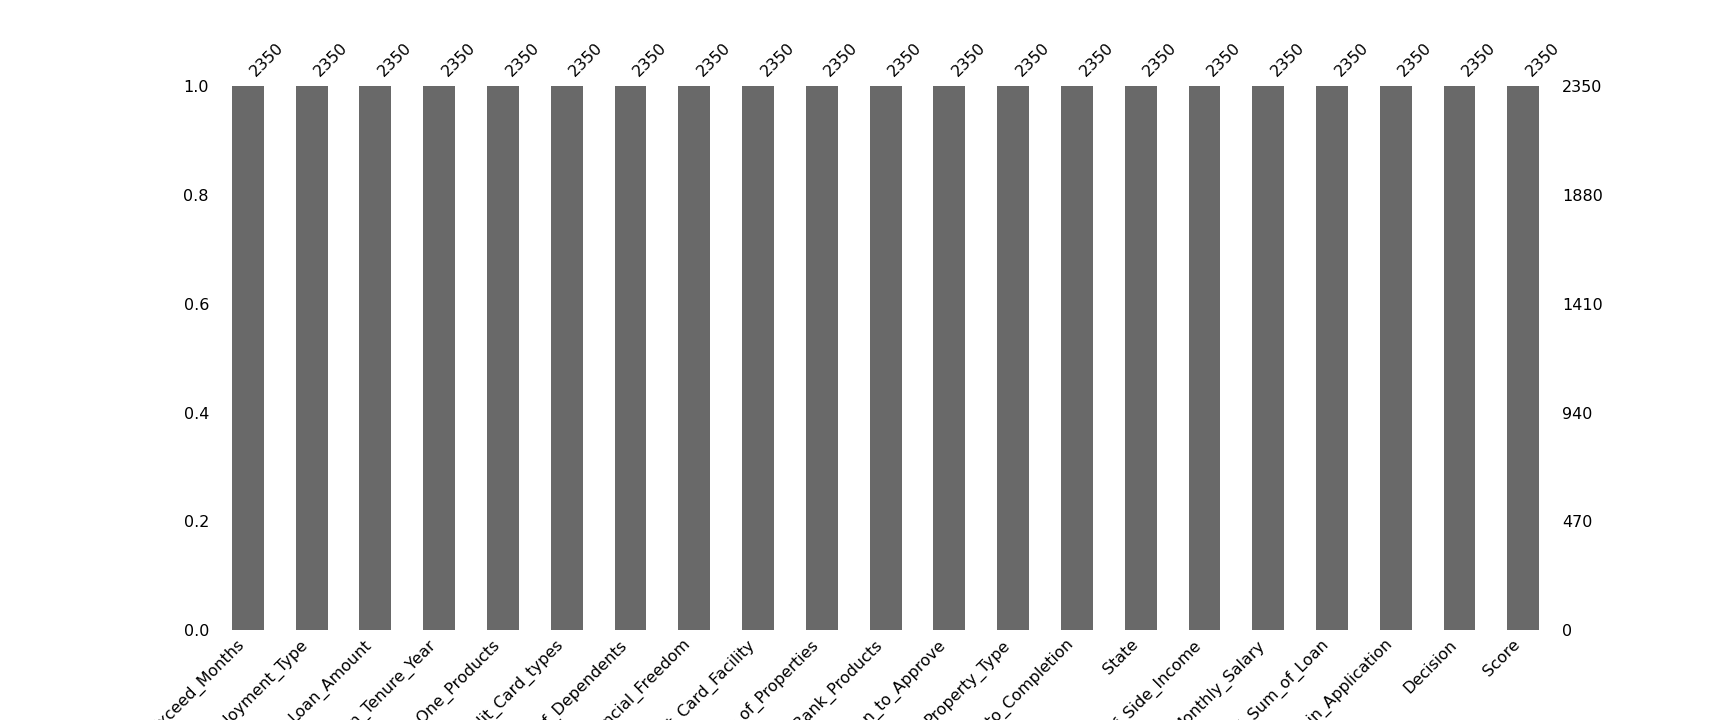
\includegraphics[scale=0.2]{filled_missing_val.png}}
\caption{The results of \textit{isnull()} after filling the mode values}
\label{fig:filledIsNull}
\end{figure}

Based on Figure~\ref{fig:filledIsNull}, we had successfully filled in the mode values to replace the missing values. All of the columns in the dataset are now containing 2350 records. 

\clearpage
\subsection{Data Pre-processing}
\subsubsection{Noisy Data}
We are going to apply regular expression (Regex) to the noisy data. Here are some of the example that we replace our data column in the dataset using Regex.

\begin{table}[ht]
\centering
\caption{\label{tab:noisyData}Noisy Data}
\begin{adjustbox}{width=.5\textwidth}
\begin{tabular}{|c|c|}
\hline
\multicolumn{1}{|l|}{\textbf{Before Regex}} & \textbf{After Regex} \\ \hline
P.Pinang  & Penang \\ \hline
Johor B  & Johor \\ \hline
K.L & Kuala Lumpur \\ \hline
N.Sembilan & Negeri Sembilan \\ \hline
SWK & Sarawak \\ \hline
Trengganu & Terrenganu \\ \hline
Self\_Employed & Self Employed \\ \hline
government & Government \\ \hline
\end{tabular}
\end{adjustbox}
\end{table}

\subsubsection{Categorizing Data}
We are going to categorize some of the data from float64 type to categorical type. We implemented \textit{.astype("category")} to categorize the data. Loan\_Amount and Monthly\_Salary are chosen to be categorized.

\clearpage
\subsection{Synthetic Minority Over-sampling Technique (SMOTE)}
\subsubsection{Imbalance Data}
In this section, we are going to oversample the imbalance data using SMOTE. We chose oversampling method is because undersampling will reduce the size of the data, thus making the dataset smaller and not enough useful data to be take into account for prediction later. 

First and foremost, we duplicated a new dataframe for SMOTE. In the new dataframe, 'Decision' is dropped and all the values are encoded using \textit{LabelEncoder()}. $X$ is the features dataframe which includes all columns except 'Decision' while $y$ is the target variable which is referring to 'Decision'. After that, $X$ and $y$ are fitted into SMOTE. 

\section{Feature Selection}
For feature selection to work, the original dataset has been transformed into an analytical dataset that is able to fit into the prediction model later on. 

Feature selection algorithms used for the dataset are Boruta and Recursive Feature Elimination (RFE). Both of the algorithms are feature ranking and selection algorithms that based on Random Forest Classifier. Due to Random Forest Classifier, both of the feature selection algorithms are able to return good accuracy and result. 

\begin{figure}[ht]
\begin{subfigure}{0.5\textwidth}
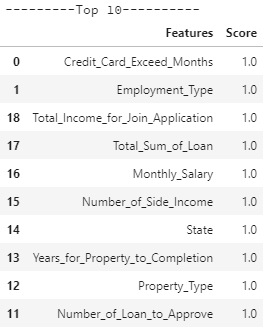
\includegraphics[scale=0.65]{BorutaTop10.PNG} 
\caption{Boruta Top 10 Features}
\label{fig:borutaTop10}
\end{subfigure}
\begin{subfigure}{0.5\textwidth}
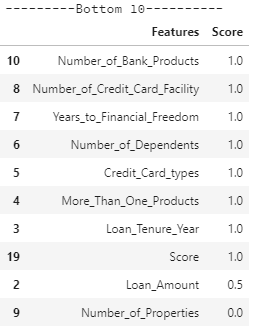
\includegraphics[scale=0.65]{BorutaBot10.PNG}
\caption{Boruta Bottom 10 Features}
\label{fig:borutaBot10}
\end{subfigure}
\label{fig:boruta}
\caption{Results of Boruta Features Selection}
\end{figure}

\clearpage
\begin{figure}[ht]
\begin{subfigure}{0.5\textwidth}
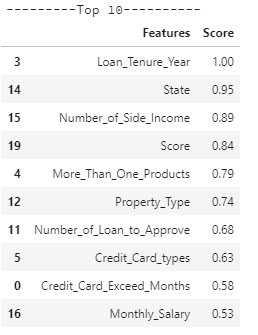
\includegraphics[scale=0.65]{RFETop10.PNG} 
\caption{RFE Top 10 Features}
\label{fig:borutaTop10}
\end{subfigure}
\begin{subfigure}{0.5\textwidth}
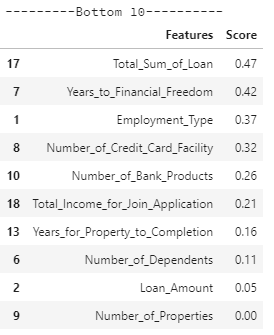
\includegraphics[scale=0.65]{RFEBot10.PNG}
\caption{RFE Bottom 10 Features}
\label{fig:borutaBot10}
\end{subfigure}
\label{fig:boruta}
\caption{Results of RFE Features Selection}
\end{figure}

Based on both of the feature selection results of Boruta and RFE, we found out that Loan$_$Amount and Number$_$of$_$Property are ranked last and having the least amount of score. We dropped both of the features and proceed into the next step. 

\clearpage
\section{Data Mining Techniques}
\subsection{Association Rule Mining}
Association rule mining is performed to extract unique rules of each individual who applies for the loan, based on the current loan duration, credit card information and amount of property the applicant have. This technique is used to investigate the combination of past loan records of the applicant. It observes the loan records that are frequently accustomed together by the applicant and calculates their strength of relations. The algorithm is suitable for this purpose because the dataset is mainly in non-numeric data. With this technique, the antecedents and consequences can be clearly identified, alongside with their scores of strength, which is measured by lift. A lift score with 1.0 and above means the combination of loan records is happening often. 

\subsection{Classification Model}
Multiple classification models are implemented to compare their performances, which are Decision Tree (DT), Naive Bayes (NB), K-Nearest Neighbor (KNN) and Support Vector Machine (SVM). These models are evaluated with multiple metrics, such as accuracy, precision, recall and F1-score. However, the metric we are going to focus on will be F1-score, as accuracy has the issue of accuracy paradox, where a model that predicts everything to be the major class will have a high accuracy. On the other hand, precision and recall only takes into consideration two classifier labels. We came to a conclusion that F1-score will be used for comparison, while other metrics can still be used as reference for more detailed breakdown of the performance of the models. 

\clearpage
\subsection{Clustering}
The dataset after the feature selection remained only categorical data, so that the clustering technique used is K-modes clustering. K-modes clustering defines clusters based on the number of matching categories between the data points, which in contrast to the K-means clustering technique that clusters the data based on a mean Euclidean distance. The Elbow Method is used in order to determine the optimal number of clusters, K. Figure~\ref{fig:kModeElbow} is plotted to compare the cost against each K. The cost is the sum of dissimilarities of all data points with their closest centroids. Based on Figure~\ref{fig:kModeElbow}, we can see that the elbow point is when K=3. Hence, the number of clusters that we used is 3.

\begin{figure}[ht]
\centerline{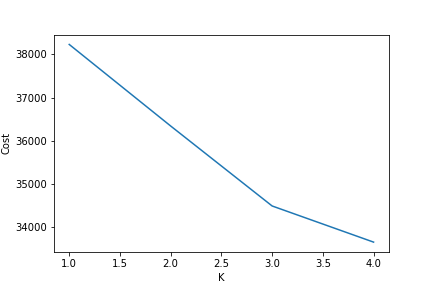
\includegraphics[scale=0.8]{kModeElbow.png} }
\label{fig:kModeElbow}
\caption{Finding the Elbow for K-Modes Clustering}
\end{figure}


\clearpage
\section{Results \& Discussion}
\subsection{Exploratory Data Analysis}
\subsubsection{Exploratory Data Analysis Before SMOTE}
In this section, we will show the Exploratory Data Analysis before applying SMOTE on the dataset. \\ \\
%=========================== EMPLOYMENT TYPE
\noindent \textbf{Question}: Which type of employment has the highest chance of getting the loan accepted?
\begin{figure}[h]
\centerline{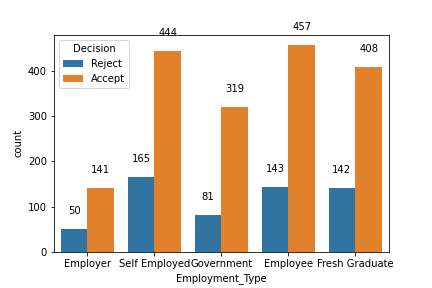
\includegraphics[scale=0.8]{bSMOTE_employment.png} }
\label{fig:bSmoteEmploy}
\caption{Employment Type before SMOTE}
\end{figure}

Figure above shows that Self Employed people have the highest count of loan application. In our opinion, this is most likely that self employed people will need the loan to start up a business. \\ \\

\clearpage
%=========================== CREDIT CARD
\noindent \textbf{Question}: Which credit card type is the most?
\begin{figure}[h]
\centerline{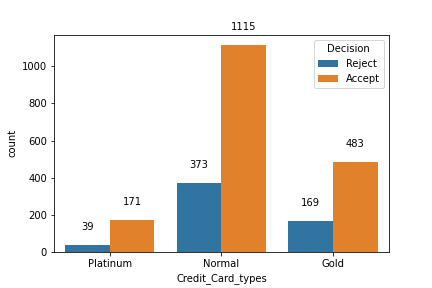
\includegraphics[scale=0.8]{bSMOTE_ccard_type.png} }
\label{fig:bSmoteCredit}
\caption{Credit card Type before SMOTE}
\end{figure}

Figure above shows that normal type of credit card user have the most loan application among platinum and gold user. In our opinion, this is most likely that normal type of credit card user will have the least amount of income compared to gold and platinum users.
\clearpage

%=========================== PROPERTY TYPE
\noindent \textbf{Question}: Which type of property type has the highest chance of getting the loan accepted?
\begin{figure}[h]
\centerline{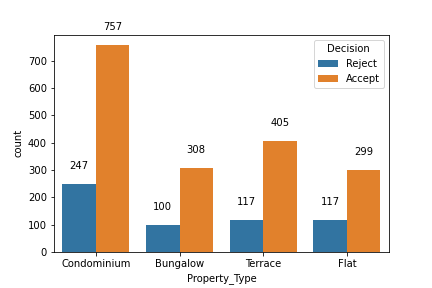
\includegraphics[scale=0.8]{bSMOTE_property.png} }
\label{fig:bSmoteProperty}
\caption{Property Type before SMOTE}
\end{figure}

Figure above shows that condominium type of property have the most loan application among the the other types. In our opinion, this is because condominium have the most average rate of income compared to other property types. For example, people who are able to afford condominium will have a more reasonable purpose to apply a loan compared to people who are staying in bungalow. 
\clearpage

%=========================== MONTH SALARY
\noindent \textbf{Question}: Which category of monthly salary has the highest chance of getting the loan accepted?
\begin{figure}[h]
\centerline{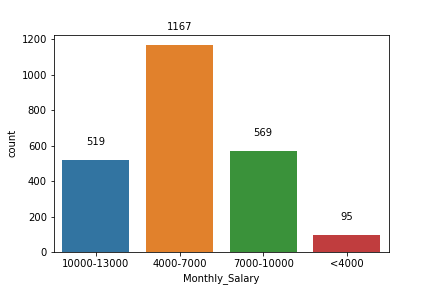
\includegraphics[scale=0.8]{bSMOTE_month_salary.png} }
\label{fig:bSmoteMonthSalary}
\caption{Monthly salary before SMOTE}
\end{figure}

Figure above shows that monthly salary category of RM4000 - RM7000 have the most loan application. In our opinion, this is because that the loan will be more helpful compared to the other categories. In the other hand, if compared to the category of less than RM4000, they will be much more helpful compared to category RM4000 - RM7000. But due to their low amount of income, they cannot guarantee that they are able to pay back the loan.
\clearpage

%=========================== DCS EMPLOYMENT
\noindent \textbf{Question}: Which type of employment has the highest chance of getting the loan accepted?
\begin{figure}[h]
\centerline{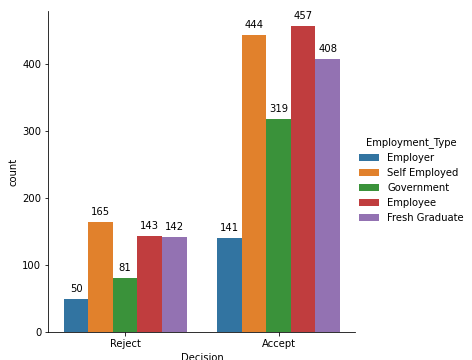
\includegraphics[scale=0.8]{bSMOTE_dcs_employment.png} }
\label{fig:bSmoteDCSemp}
\caption{Bank decision on employment type before SMOTE}
\end{figure}

Figure above shows that Employee have the most acceptance counts compared to the other employment type. In our opinion, this is because that employee have a more stable income compared to the other employment type. For example, self employed people will have a higher risk of losing their own business.
\clearpage

%=========================== DCS CREDIT CARD
\noindent \textbf{Question}: Which type of credit card has the highest chance of getting the loan accepted?
\begin{figure}[h]
\centerline{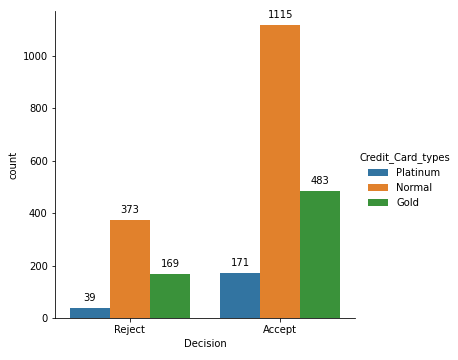
\includegraphics[scale=0.8]{bSMOTE_dcs_ccard_type.png} }
\label{fig:bSmoteDSCcc}
\caption{Bank decision on credit card type before SMOTE}
\end{figure}

Figure above shows that normal type of credit card users have the highest acceptance count compared to the other types. In our opinion, this is because that accepting normal credit card user will be more helpful for them them compared to the other types of credit card users.
\clearpage

%=========================== DCS PROPERTY TYPE
\noindent \textbf{Question}: Which type of property has the highest chance of getting the loan accepted?
\begin{figure}[h]
\centerline{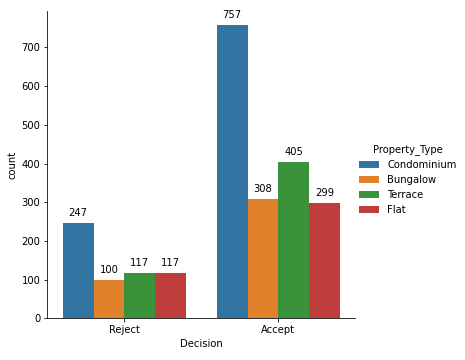
\includegraphics[scale=0.8]{bSMOTE_dcs_property.png} }
\label{fig:bSmoteDCSproperty}
\caption{Bank decision on property type before SMOTE}
\end{figure}

Figure above shows that condominium property type have the highest acceptance count compared to the other property type. In our opinion, this is because that people who are able to afford condominium will have an average and stable income compared to those who are staying in terrace and flat. In the other hand, people who are living in bungalow are probably those who does not need loan and people who are living in terrace and flat have the risk of not able to pay back the loan on time.
\clearpage

%=========================== DCS MONTH SALARY
\noindent \textbf{Question}: Which category of monthly salary has the highest chance of getting the loan accepted?
\begin{figure}[h]
\centerline{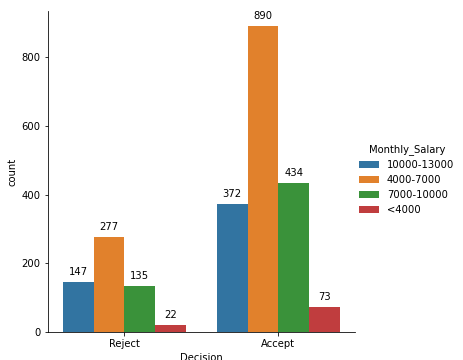
\includegraphics[scale=0.8]{bSMOTE_dcs_month_salary.png} }
\label{fig:bSmoteDCSmonthsalary}
\caption{Bank decision on monthly salary category before SMOTE}
\end{figure}

Figure above shows that monthly salary category of RM4000 - RM7000 have the most acceptance rate compared to the other categories. In our opinion, this is because that accepting those who are in the category of RM4000 - RM7000 will be more helpful compared to the other categories. In the other hand, for the bank to accept those who are in the category of lesser than RM4000 will have the risk of them could not payback the loan because of their low monthly salary.
\clearpage

%=========================== DCS MONTH SALARY
\noindent \textbf{Question}: Which decision is made most?
\begin{figure}[h]
\centerline{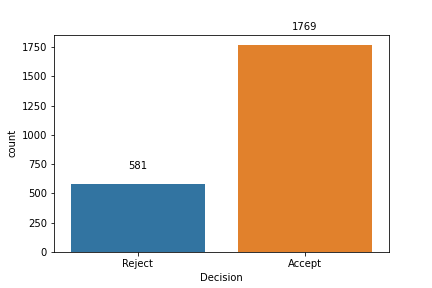
\includegraphics[scale=0.8]{bSMOTE_dcs_bank.png} }
\label{fig:bSmoteDCSbank}
\caption{Bank decision before SMOTE}
\end{figure}

Figure above shows that the bank accept most loan application. Based on the dataset and the data we visualized, we found out that the in each of the features, such as employment type, monthly salary, credit card types and property type. All of these features are being treated as the factors for loan acceptance. Thus, resulting in the bank having higher acceptance rate compared to rejection rate in terms of decision-making in loan application. 
\clearpage

%==============================================================================%

\subsubsection{Exploratory Data Analysis After SMOTE}
In this section, we will show the Exploratory Data Analysis after applying SMOTE on the dataset. \\
%=========================== EMPLOYMENT TYPE
\noindent \textbf{Question}: Which type of employment has the highest chance of getting the loan accepted?
\begin{figure}[h]
\centerline{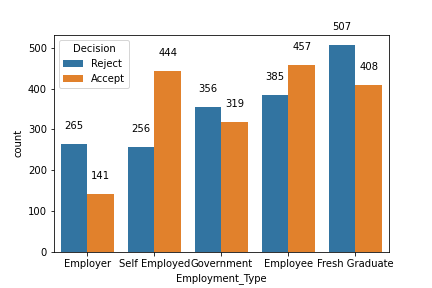
\includegraphics[scale=0.8]{aSMOTE_employment.png} }
\label{fig:aSmoteEmploy}
\caption{Employment Type after SMOTE}
\end{figure}

Figure above shows the employment type after applying SMOTE. Comparing with figure 3, we are able to observe that the number of fresh graduates had increased and became the most among the other employment type.
\clearpage

%=========================== CREDIT CARD
\noindent \textbf{Question}: Which type of credit card has the highest chance of getting the loan accepted?
\begin{figure}[h]
\centerline{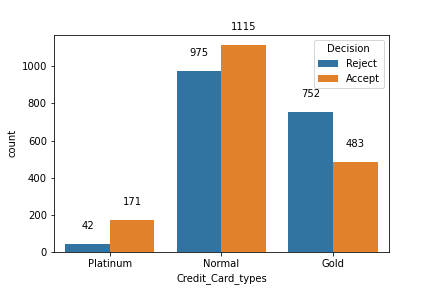
\includegraphics[scale=0.8]{aSMOTE_ccard_type.png} }
\label{fig:aSmoteCredit}
\caption{Credit card Type after SMOTE}
\end{figure}

Figure above shows the credit card type after applying SMOTE. Comparing with figure 4, we are able to observe that there is a light increment on normal and gold users.
\clearpage

%=========================== PROPERTY TYPE
\noindent \textbf{Question}: Which type of property has the highest chance of getting the loan accepted?
\begin{figure}[h]
\centerline{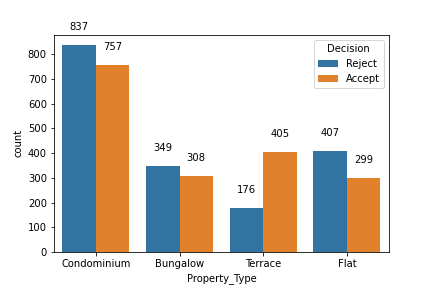
\includegraphics[scale=0.8]{aSMOTE_property.png} }
\label{fig:aSmoteProperty}
\caption{Property Type after SMOTE}
\end{figure}

Figure above shows the property type after applying SMOTE, Comparing with figure 5, we can observe that the number of terrace had increased by a little.
\clearpage

%=========================== MONTH SALARY
\noindent \textbf{Question}: Which category of monthly salary has the highest chance of getting the loan accepted?
\begin{figure}[h]
\centerline{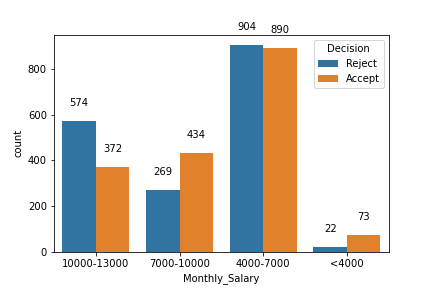
\includegraphics[scale=0.8]{aSMOTE_month_salary.png} }
\label{fig:aSmoteMonthSalary}
\caption{Monthly salary after SMOTE}
\end{figure}

Figure above shows the property type after applying SMOTE. Comparing with figure 6, we are able to observe that there is an increment at the category RM4000 - RM7000 and RM10000 - RM13000.
\clearpage

%=========================== DCS EMPLOYMENT
\noindent \textbf{Question}: Which type of employment has the highest chance of getting the loan accepted?
\begin{figure}[h]
\centerline{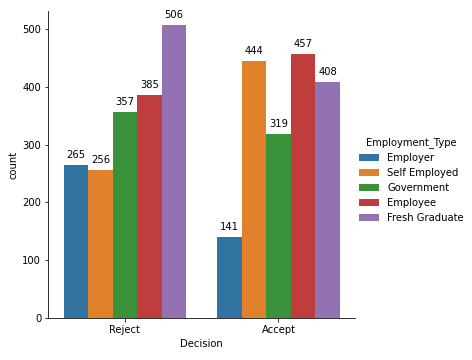
\includegraphics[scale=0.8]{aSMOTE_dcs_employment.png} }
\label{fig:aSmoteDCSemp}
\caption{Bank decision on employment type after SMOTE}
\end{figure}

Figure above shows the loan acceptance and rejection by the employment type. Comparing to figure 7, we can observe that the number of rejected loan applications had greatly decreased.
\clearpage

%=========================== DCS CREDIT CARD
\noindent \textbf{Question}: Which type of credit card has the highest chance of getting the loan accepted?
\begin{figure}[h]
\centerline{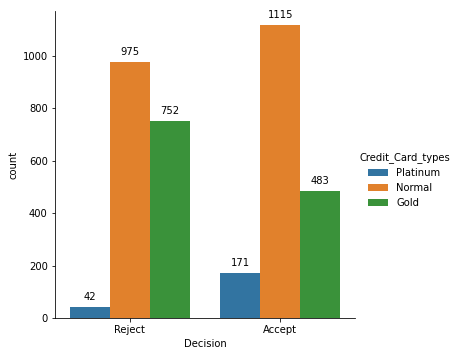
\includegraphics[scale=0.8]{aSMOTE_dcs_ccard_type.png} }
\label{fig:aSmoteDSCcc}
\caption{Bank decision on credit card type after SMOTE}
\end{figure}

Figure above shows the loan acceptance and rejection by credit card types. Comparing to figure 8, we are able to observe that the number of rejected loan applications had greatly decreased.
\clearpage

%=========================== DCS PROPERTY TYPE
\noindent \textbf{Question}: Which type of property has the highest chance of getting the loan accepted?
\begin{figure}[h]
\centerline{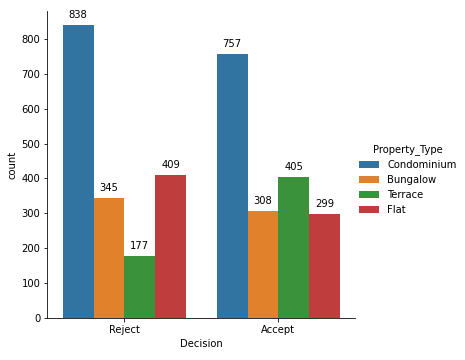
\includegraphics[scale=0.8]{aSMOTE_dcs_property.png} }
\label{fig:aSmoteDCSproperty}
\caption{Bank decision on property type after SMOTE}
\end{figure}

Figure above shows the loan acceptance and rejection by property types. Comparing to figure 9, we can observe that the number of rejected loan application on condominium had greatly decreased.
\clearpage

%=========================== DCS MONTH SALARY
\noindent \textbf{Question}: Which category of monthly salary has the highest chance of getting the loan accepted?
\begin{figure}[h]
\centerline{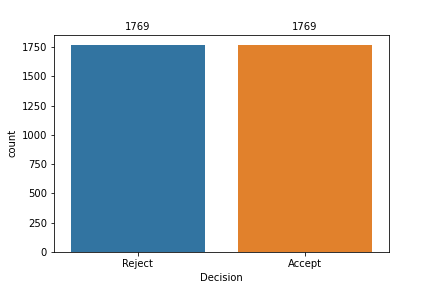
\includegraphics[scale=0.8]{aSMOTE_dcs_month_salary.png} }
\label{fig:aSmoteDCSmonthsalary}
\caption{Bank decision on monthly salary category after SMOTE}
\end{figure}

Figure above shows the loan acceptance and rejection by monthly salary. Comparing to figure 10, we are able to observe that the number of rejected applications on category RM4000 - RM7000 had greatky decreased.
\clearpage

%=========================== DCS MONTH SALARY
\noindent \textbf{Question}: Which decision is made most?
\begin{figure}[h]
\centerline{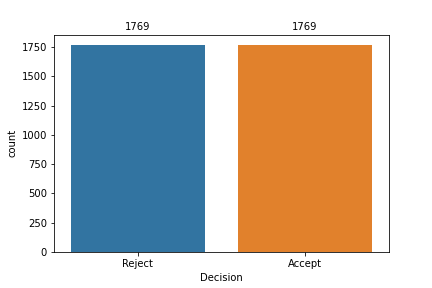
\includegraphics[scale=0.8]{aSMOTE_dcs_bank.png} }
\label{fig:aSmoteDCSbank}
\caption{Bank decision after SMOTE}
\end{figure}

Figure above shows the total number of loan acceptance and rejection by the bank. Comparing to figure 11, we can observe that the number is balanced out on both reject and accept.
\clearpage

%============================================%


\subsection{Association Rule Mining}
\begin{figure}[h]
\centerline{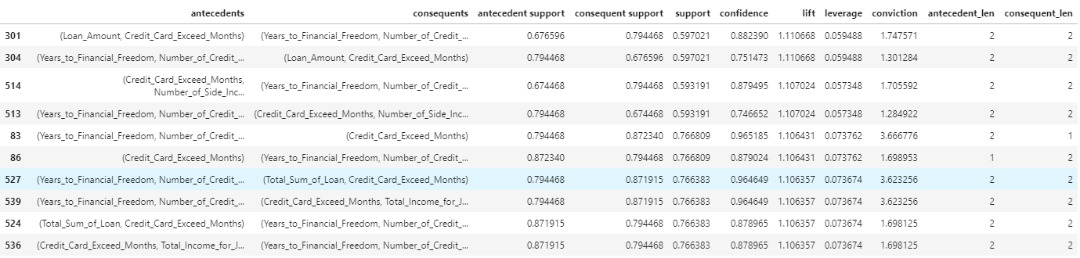
\includegraphics[scale=0.35]{armResults.jpeg}}
\caption{Antecedents and Consequences of Association Rules Mining}
\label{fig:armResults}
\end{figure}

The association rule mining algorithm can be adjusted by setting different minimum thresholds for support, confidence and lift as well as setting the numbers of antecedents and consequences. Based on Figure~\ref{fig:armResults}, the minimum support and confidence is set at 0.5, with a lift score at least 1.0, and at most 2 antecedents and consequences. The rules are also sorted by lift score. Based on the results in Figure~\ref{fig:armResults},  we found out that most of the applicant which are experiencing financial freedom in recent years are tend to have different credit card facilities. This is probably due to those applicant had stable income, so that they can apply different credit cards. 

\subsection{Classification Models}
In this section, we are going to explore each classification model in detail. We will perform evaluation scores on each classification model and seek for the best F1-score to be used for our prediction model.

\clearpage
\subsubsection{Decision Tree (DT)}
\begin{table}[ht]
\centering
\caption{\label{tab:dtMetrics}Evaluation Scores of the Decision Tree model}
\begin{adjustbox}{width=0.7\textwidth}
\begin{tabular}{|c|c|c|c|c|}
\hline
\textbf{} & \textbf{Accuracy} & \textbf{Precision} & \textbf{Recall} & \textbf{F1-Score} \\ \hline
DT        & 0.684557          & 0.683186           & 0.712177        & 0.697380          \\ \hline
\end{tabular}
\end{adjustbox}
\end{table}

\begin{figure}[ht]
\begin{subfigure}{0.5\textwidth}
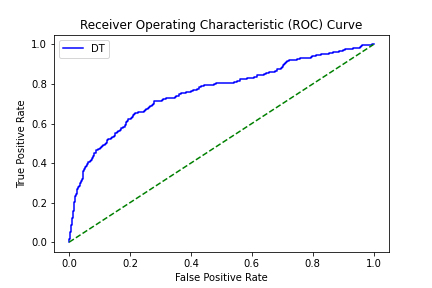
\includegraphics[scale=0.45]{roc_dt.png} 
\caption{ROC Curve}
\label{fig:rocDT}
\end{subfigure}
\begin{subfigure}{0.5\textwidth}
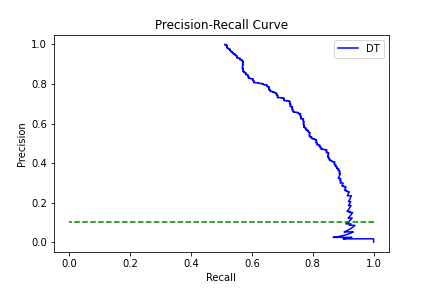
\includegraphics[scale=0.45]{prs_dt.png}
\caption{Precision-Recall Curve}
\label{fig:prsDT}
\end{subfigure}
\label{fig:csDT}
\caption{Curve Scores of Decision Tree}
\end{figure}

\clearpage
\subsubsection{Naive Bayes (NB)}
\begin{table}[ht]
\centering
\caption{\label{tab:nbMetrics}Evaluation Scores of the Naive Bayes model}
\begin{adjustbox}{width=0.7\textwidth}
\begin{tabular}{|c|c|c|c|c|}
\hline
\textbf{} & \textbf{Accuracy} & \textbf{Precision} & \textbf{Recall} & \textbf{F1-Score} \\ \hline
NB        & 0.713747          & 0.722846           & 0.712177        & 0.717472          \\ \hline
\end{tabular}
\end{adjustbox}
\end{table}

\begin{figure}[ht]
\begin{subfigure}{0.5\textwidth}
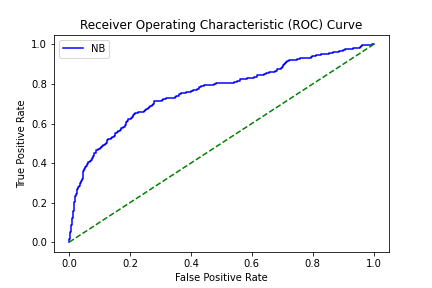
\includegraphics[scale=0.45]{roc_nb.png} 
\caption{ROC Curve}
\label{fig:rocNB}
\end{subfigure}
\begin{subfigure}{0.5\textwidth}
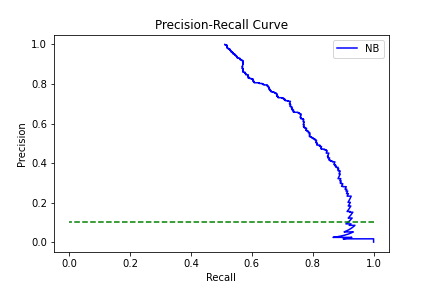
\includegraphics[scale=0.45]{prs_nb.png}
\caption{Precision-Recall Curve}
\label{fig:prsNB}
\end{subfigure}
\label{fig:csNB}
\caption{Curve Scores of Naive Bayes}
\end{figure}

\clearpage
\subsubsection{K-Nearest Neighbor (KNN)}
\begin{table}[ht]
\centering
\caption{\label{tab:knnMetrics}Evaluation Scores of the K-Nearest Neighbor model}
\begin{adjustbox}{width=0.7\textwidth}
\begin{tabular}{|c|c|c|c|c|}
\hline
\textbf{KNN} & \textbf{Accuracy} & \textbf{Precision} & \textbf{Recall} & \textbf{F1-Score} \\ \hline
K=3        & 0.661016          & 0.646774           & 0.739852        & 0.690189          \\ \hline
K=6        & 0.621468          & 0.643442           & 0.579335        & 0.609708          \\ \hline
K=9        & 0.612052          & 0.610544           & 0.662361        & 0.635398          \\ \hline
\end{tabular}
\end{adjustbox}
\end{table}

\begin{figure}[ht]
\centerline{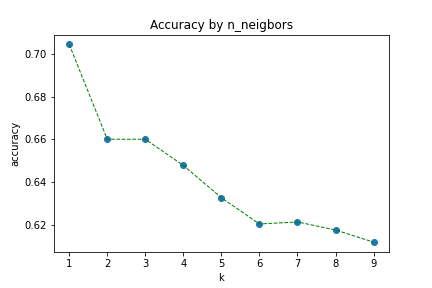
\includegraphics[scale=0.35]{knn_plot.png}}
\label{fig:knnPlot}
\caption{Accuracy by n-neighbors}
\end{figure}

\begin{figure}[ht]
\begin{subfigure}{0.5\textwidth}
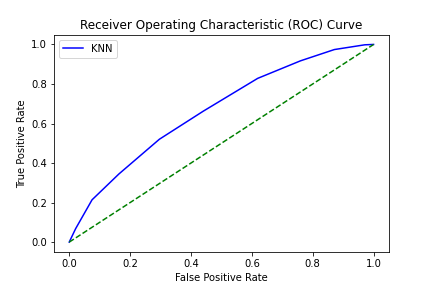
\includegraphics[scale=0.45]{roc_knn.png} 
\caption{ROC Curve}
\label{fig:rocKNN}
\end{subfigure}
\begin{subfigure}{0.5\textwidth}
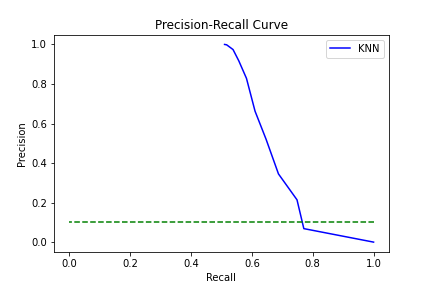
\includegraphics[scale=0.45]{prs_knn.png}
\caption{Precision-Recall Curve}
\label{fig:prsKNN}
\end{subfigure}
\label{fig:csKNN}
\caption{Curve Scores of K-Nearest Neighbor}
\end{figure}

\clearpage
\subsubsection{Support Vector Machine (SVM)}
\begin{table}[ht]
\centering
\caption{\label{tab:svmMetrics}Evaluation Scores of the Support Vector Machine model}
\begin{adjustbox}{width=0.7\textwidth}
\begin{tabular}{|c|c|c|c|c|}
\hline
\textbf{SVM Kernel} & \textbf{Accuracy} & \textbf{Precision} & \textbf{Recall} & \textbf{F1-Score} \\ \hline
Rbf        & 0.694915          & 0.932539           & 0.433579        & 0.592686          \\ \hline
Linear        & 0.671374          & 0.689587           & 0.647601        & 0.667935          \\ \hline
\end{tabular}
\end{adjustbox}
\end{table}

Due to hardware and system constraint, we are unable to perform Linear and Poly kernel for Support Vector Machine. For Linear kernel, we are able to retrieve the evaluation score after 2 hours. As for Poly kernel, we failed to retrieve any evaluation score even after one day. Due to the execution time is high, we are utilizing Rbf kernel as our representation for Support Vector Machine.

\begin{figure}[ht]
\begin{subfigure}{0.5\textwidth}
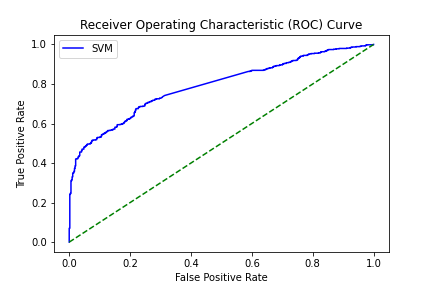
\includegraphics[scale=0.45]{roc_svm.png} 
\caption{ROC Curve}
\label{fig:rocSVM}
\end{subfigure}
\begin{subfigure}{0.5\textwidth}
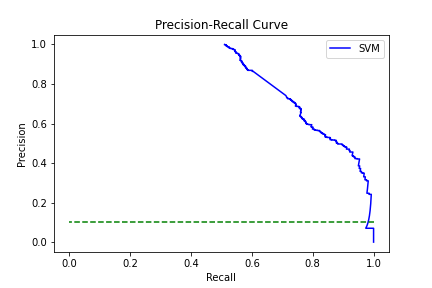
\includegraphics[scale=0.45]{prs_svm.png}
\caption{Precision-Recall Curve}
\label{fig:prsSVM}
\end{subfigure}
\label{fig:csSVM}
\caption{Curve Scores of Support Vector Machine}
\end{figure}

\clearpage
\subsubsection{Classification Evaluation Model}
\begin{table}[ht]
\centering
\caption{\label{tab:f1Metrics}F1-Score of the classification models}
\begin{adjustbox}{width=.5\textwidth}
\begin{tabular}{|c|c|c|c|c|}
\hline
\textbf{Classification Model} & \textbf{F1-Score}\\ \hline
Decision Tree & 0.697380 \\ \hline
Naive Bayes & 0.717472 \\ \hline
K-Nearest Neighbor & 0.690189 \\ \hline
Support Vector Machine & 0.592686\\ \hline
\end{tabular}
\end{adjustbox}
\end{table}

\begin{figure}[h]
\centerline{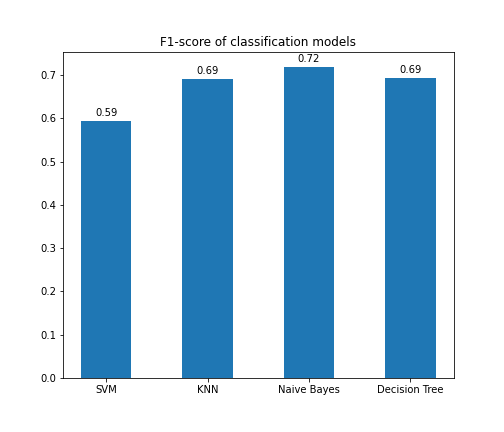
\includegraphics[scale=0.65]{classificationModel.png}}
\caption{F1-Score of Classification Models}
\label{fig:modelEvaluation}
\end{figure}

Based on Figure ~\ref{fig:modelEvaluation}, we found out that Naive Bayes have the highest score in terms of F1-Score. So, we implemented Naive Bayes as the machine learning model for our prediction model later on. 

\begin{table}[ht]
\centering
\caption{\label{tab:f1Metrics}Table of Comparison between all AUC and Precision-Recall Curves}
\begin{adjustbox}{width=1\textwidth}
\begin{tabular}{|c|c|c|c|c|}
\hline
\textbf{Classification Model} & \textbf{AUC} & \textbf{Precision-Recall Curve}\\ \hline
Decision Tree & 0.76 & 0.78\\ \hline
Naive Bayes & 0.76 & 0.78\\ \hline
K-Nearest Neighbor & 0.66 & 0.64\\ \hline
Support Vector Machine & 0.79 & 0.83\\ \hline
\end{tabular}
\end{adjustbox}
\end{table}

\begin{figure}[ht]
\begin{subfigure}{0.5\textwidth}
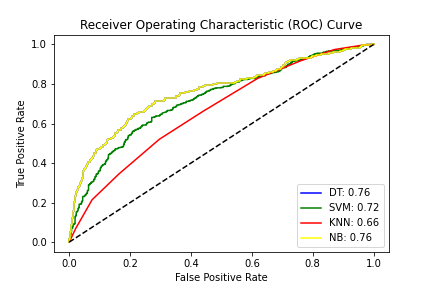
\includegraphics[scale=0.45]{roc_all.png} 
\caption{ROC Curve}
\label{fig:rocAll}
\end{subfigure}
\begin{subfigure}{0.5\textwidth}
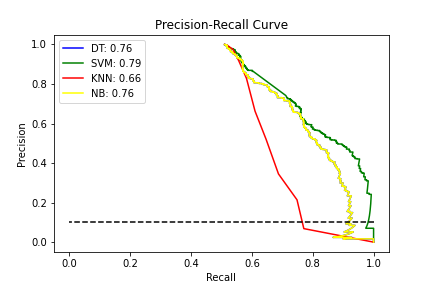
\includegraphics[scale=0.45]{prs_all.png}
\caption{Precision-Recall Curve}
\label{fig:prsAll}
\end{subfigure}
\label{fig:csAll}
\caption{Curve Scores of all Classification Models}
\end{figure}

\clearpage
\subsection{Clustering}
\subsubsection{K-Modes Clustering}

\begin{figure}[h]
\centerline{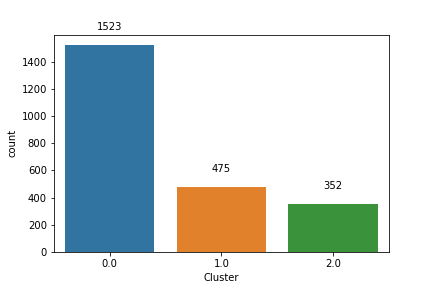
\includegraphics[scale=0.65]{kmodeCluster.png}}
\caption{Cluster after performing K-Modes Clustering}
\label{fig:kModeCluster}
\end{figure}

Based on Figure ~\ref{fig:kModeCluster}, we can then visualize more in depth into the features we will be using in the prediction model. Cluster 0 occupied the most proportions compared to Cluster 1 and Cluster 2. All of the Cluster 0s have a larger proportion compared to their respective Cluster 1 and Cluster 2.
\begin{figure}[h]
\centerline{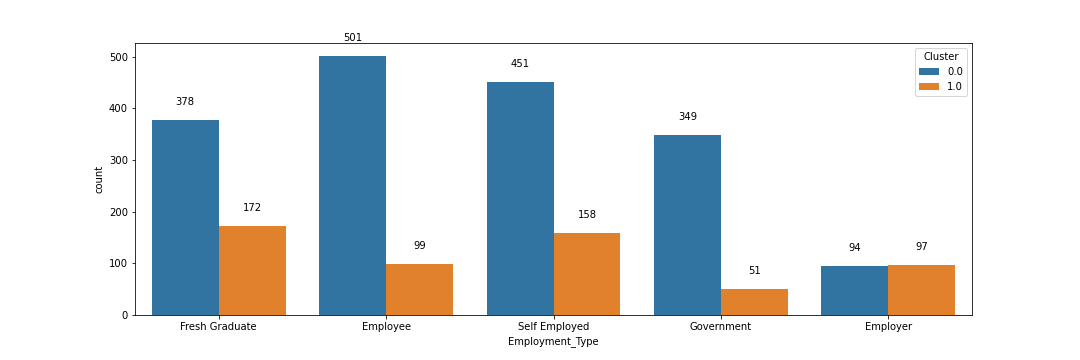
\includegraphics[scale=0.5]{kmode_employ.png}}
\label{fig:kModeEmploy}
\caption{K-Modes Clustering of Employment Type}
\end{figure}
\begin{figure}[h]
\centerline{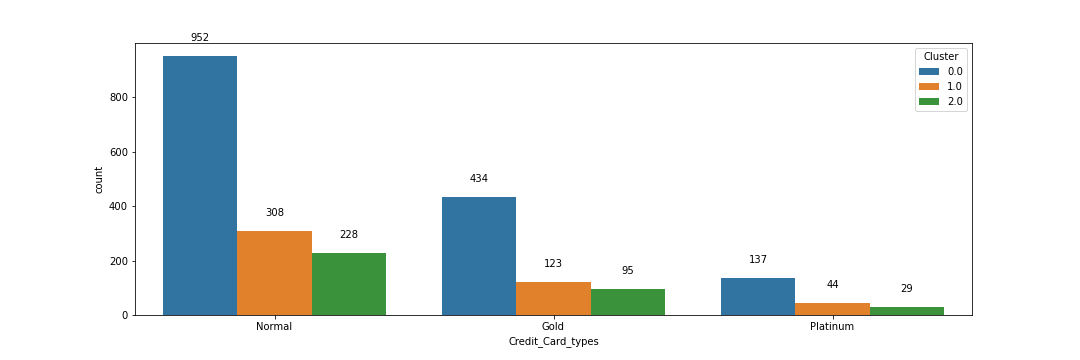
\includegraphics[scale=0.5]{kmode_ccard.png}}
\label{fig:kModeEmploy}
\caption{K-Modes Clustering of Credit Card Type}
\end{figure}
\begin{figure}[h]
\centerline{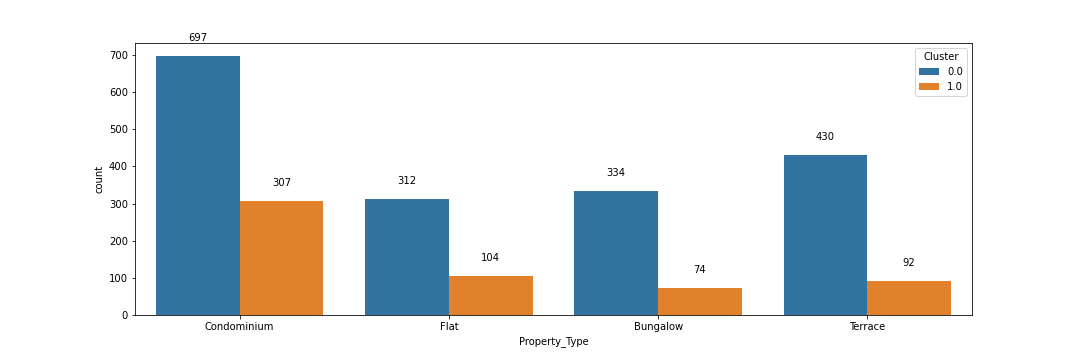
\includegraphics[scale=0.5]{kmode_property.png}}
\label{fig:kModeEmploy}
\caption{K-Modes Clustering of Property Type}
\end{figure}
\begin{figure}[h]
\centerline{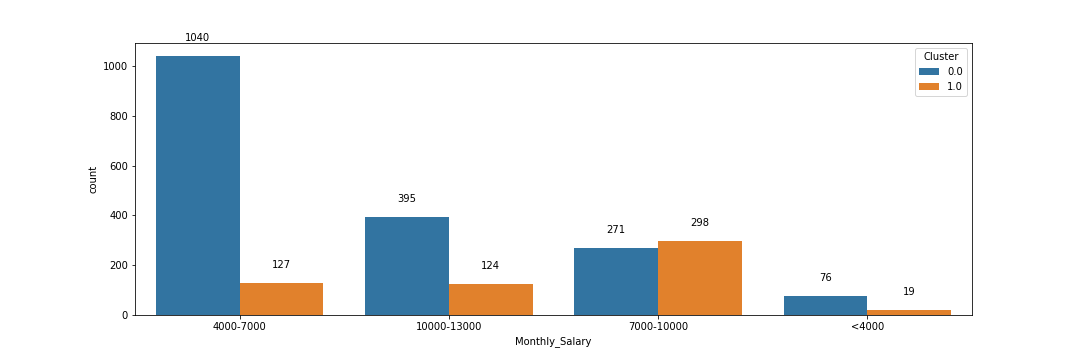
\includegraphics[scale=0.5]{kmode_salary.png}}
\label{fig:kModeEmploy}
\caption{K-Modes Clustering of Monthly Salary}
\end{figure}

\clearpage
\subsection{Conclusion}
From the data mining tasks executed above, multiple findings about the banking data have been discovered, such as which employment type apply for loan the most, how much of the monthly salary required to apply for loan, which type of credit card user will apply for loan the most and much more. Besides that, multiple classification models have been built to predict the `Decision' based on the applicant's loan records. At the end, the result of the Naive Bayes model provides the highest F1-score. Thus, for our prediction model, we will be implementing Naive Bayes as our model for training and predicting the dataset. Besides that, the K-modes clustering technique is also performed on the dataset.  

\clearpage
\section{Deployment}
For deployment, we implemented Tkinter to create our prediction model. Tkinter is an integrated library which comes along with python. Upon landing page, the user is able to select ARM, EDA, Machine Learning Techiniques, Clustering and Prediction Model from the title bar. To run the program, the user would need to open it up in the command prompt and type in \textbf{python3 Project.py}. After that, Figure~\ref{fig:deployPm} will be displayed.

\begin{figure}[h]
\centerline{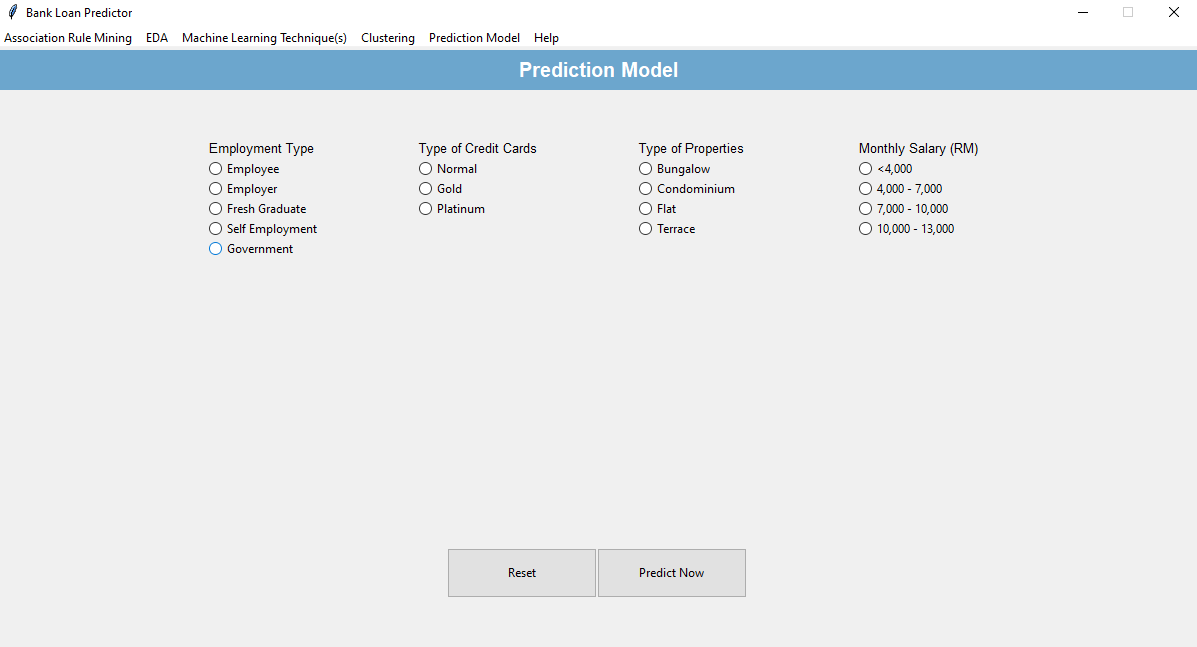
\includegraphics[scale=0.35]{deploy_pm.PNG}}
\caption{Prediction Model}
\label{fig:deployPm}
\end{figure}

\clearpage

When the user click on the EDA tab, the user will be able to view the visualization of the data before and after applying SMOTE.

\begin{figure}[h]
\centerline{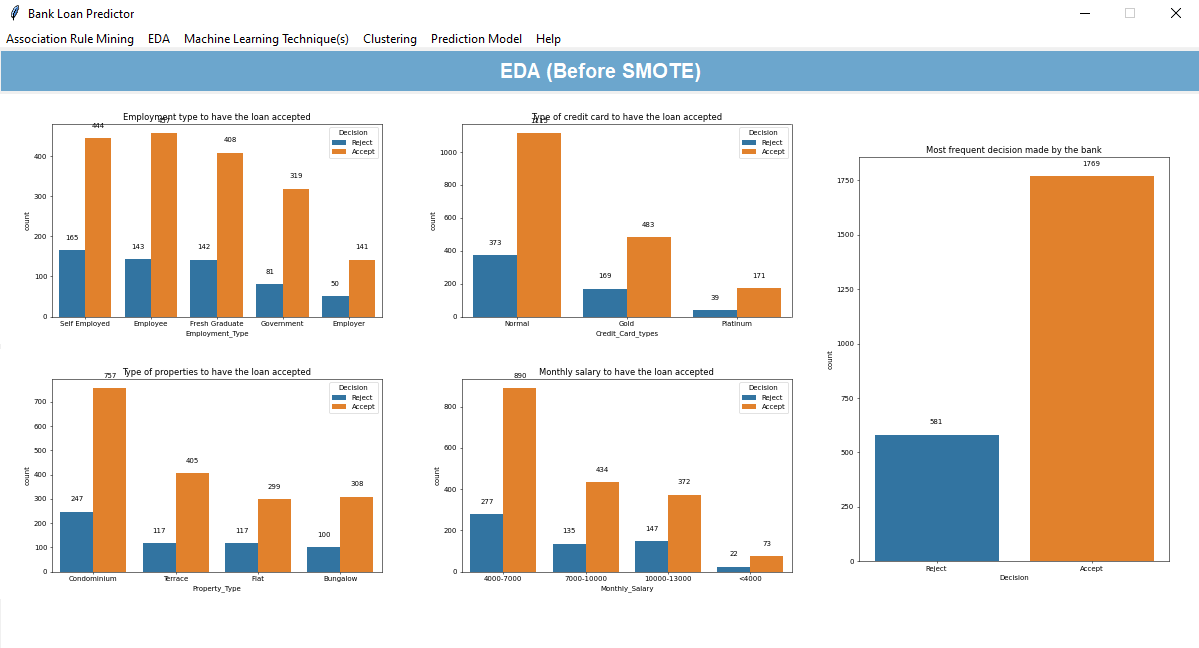
\includegraphics[scale=0.35]{deploy_b4Smote.PNG}}
\label{fig:deployBsmote}
\caption{Before Smote}
\end{figure}

\begin{figure}[h]
\centerline{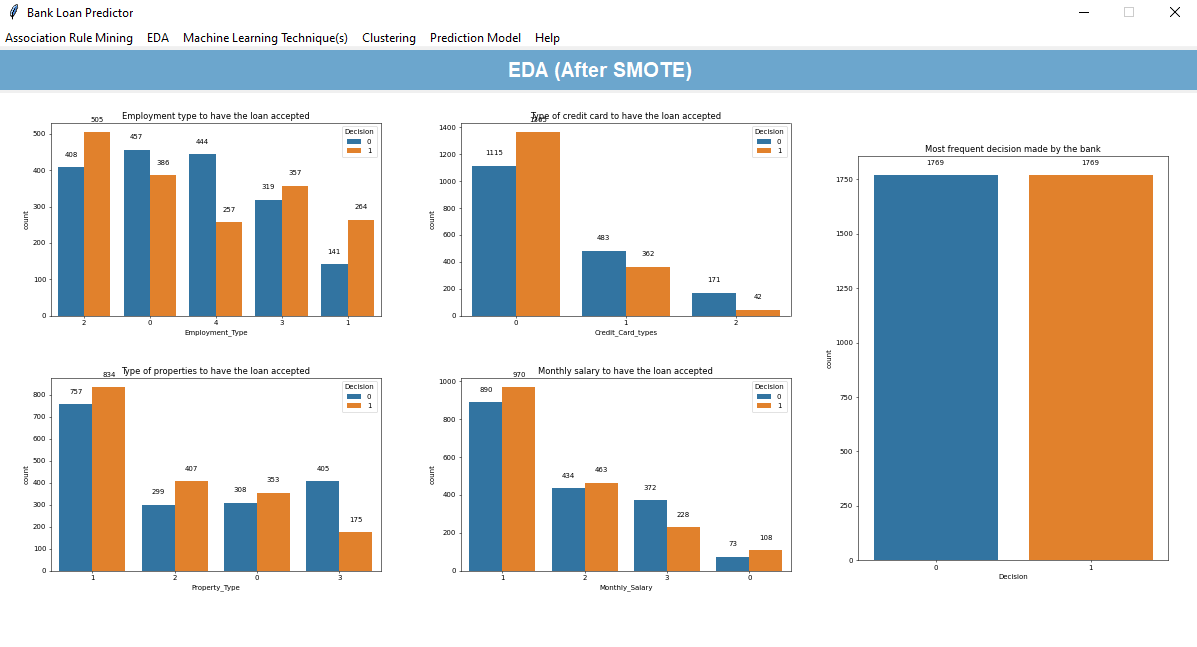
\includegraphics[scale=0.35]{deploy_smote.PNG}}
\label{fig:deployARM}
\caption{After Smote}
\end{figure}

\clearpage

On the Association Rule Mining tab, the user will be able to set the minimum support, minimum confidence, minimum lift, number of antecedent and number of consequent. After selecting all those parameters, the user can generate the rule by clicking the "Generate Rules" button.

\begin{figure}[h]
\centerline{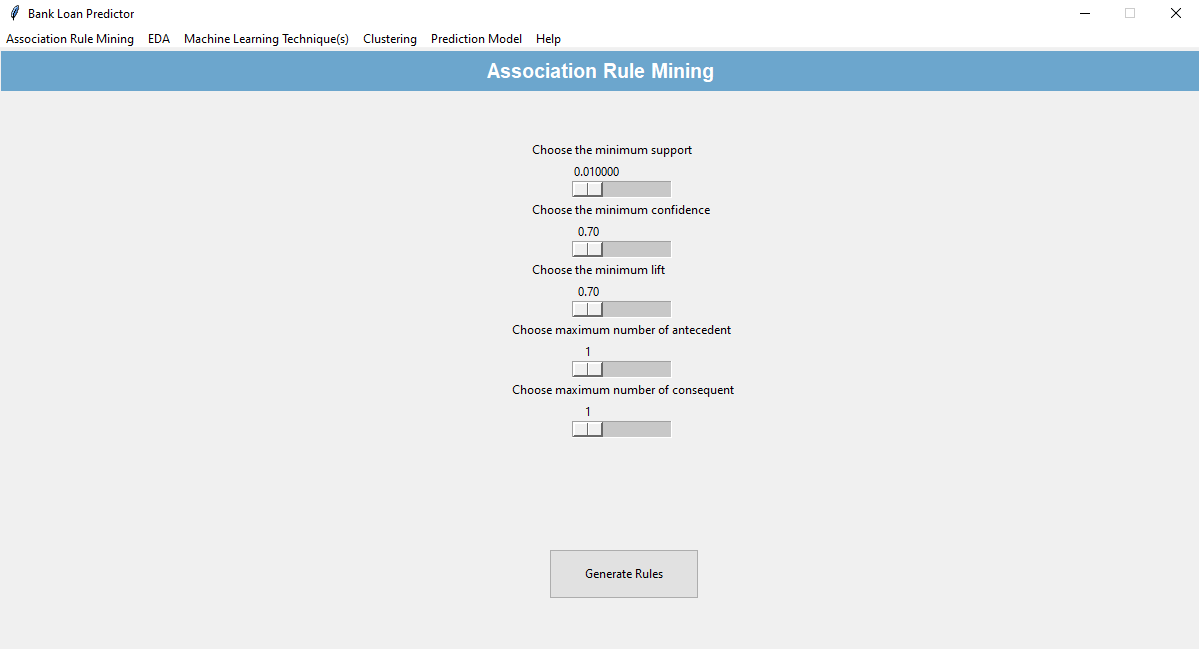
\includegraphics[scale=0.35]{deploy_arm.PNG}}
\label{fig:deployARM}
\caption{Association Rule Mining}
\end{figure}

\begin{figure}[h]
\centerline{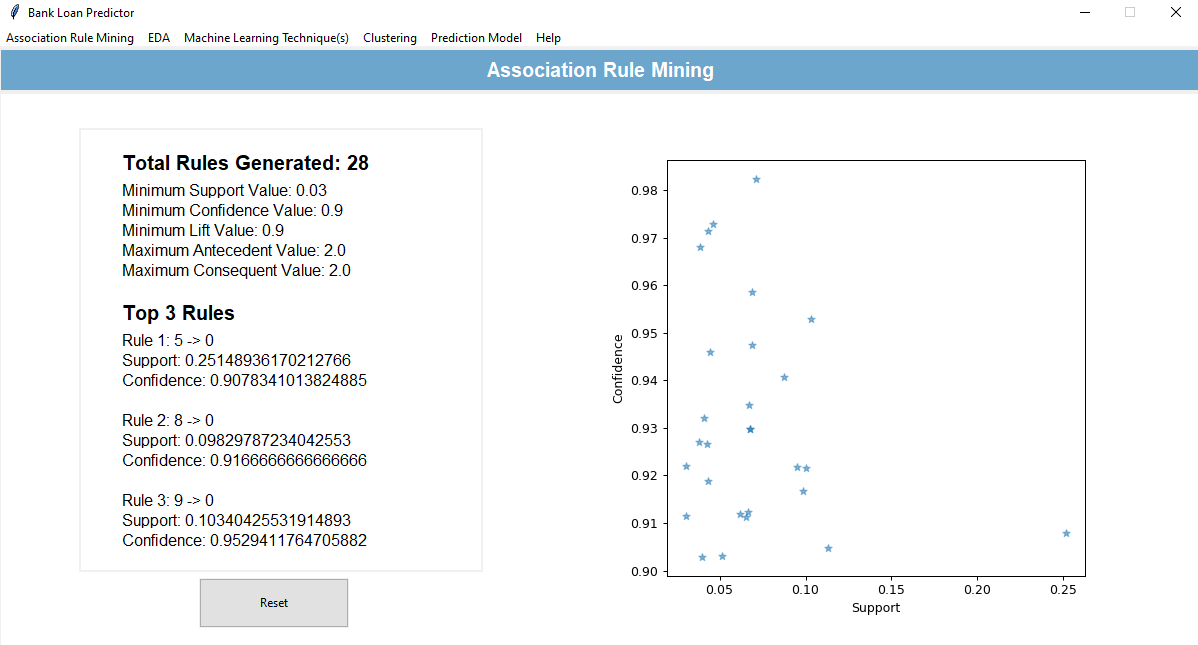
\includegraphics[scale=0.35]{deploy_armResults.PNG}}
\label{fig:deployARM-2}
\caption{ARM after}
\end{figure}

\clearpage

On the Machine Learning Technique tab, the user are able to choose machine learning techniques such as SVM, KNN, Naive Bayes and Decision Tree. After selecting the ML techniques, the user will be able to view the Receiver Operating Characteristic curve, Precision-Recall Curve and F1-score of classification models.

\begin{figure}[h]
\centerline{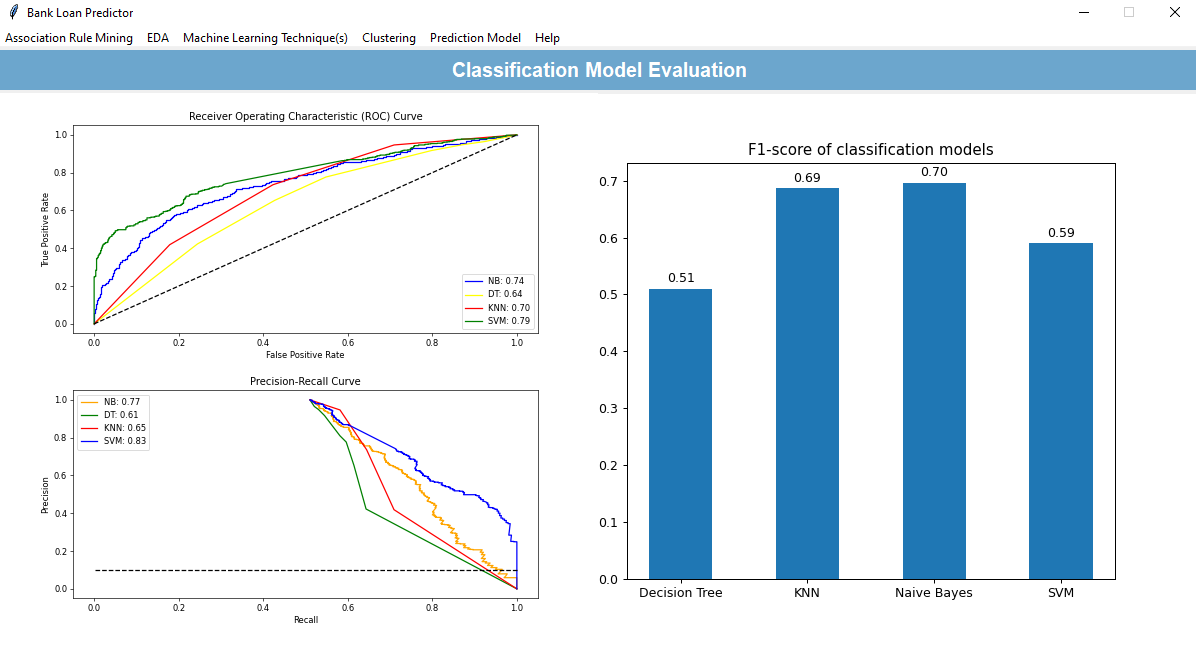
\includegraphics[scale=0.35]{deploy_cme.PNG}}
\label{fig:deployCME}
\caption{Classification Model Evaluation}
\end{figure}

\begin{figure}[h]
\centerline{\includegraphics[scale=0.35]{deploy_knn.PNG}}
\label{fig:deployKNN}
\caption{K-Nearest Neighbour}
\end{figure}

\begin{figure}[h]
\centerline{\includegraphics[scale=0.35]{deploy_nb.PNG}}
\label{fig:deployNB}
\caption{Naive Bayes}
\end{figure}

\begin{figure}[h]
\centerline{\includegraphics[scale=0.35]{deploy_svm.PNG}}
\label{fig:deploysvm}
\caption{Support Vector Machine}
\end{figure}

\clearpage

On the clustering tab, the user will be able to view the visualization of the K-Nearest NeighBour. By changing the sliding bar, the visualized data will be able to change immediately.

\begin{figure}[h]
\centerline{\includegraphics[scale=0.35]{deploy_kmodes.PNG}}
\label{fig:deployKmodes}
\caption{K-Modes Clustering}
\end{figure}

\pagenumbering{gobble} 
\end{document}